% ============================================================
%  SESSION 4 — React Derinleşme
%  XeLaTeX ile derleyin: xelatex session-04.tex
% ============================================================
\documentclass[12pt, a4paper]{article}

% ---------- Font & Dil ----------
\usepackage{fontspec}
\usepackage[turkish, shorthands=off]{babel}
\setmainfont{Georgia}
\setsansfont{Arial}
\setmonofont{Courier New}

% ---------- Sayfa Düzeni ----------
\usepackage[top=2.2cm, bottom=2.2cm, left=2.4cm, right=2.4cm]{geometry}
\usepackage{parskip}
\setlength{\parindent}{0pt}

% ---------- Renkler ----------
\usepackage{xcolor}
\definecolor{primary}{HTML}{2563EB}
\definecolor{secondary}{HTML}{7C3AED}
\definecolor{accent}{HTML}{059669}
\definecolor{warning}{HTML}{D97706}
\definecolor{danger}{HTML}{DC2626}
\definecolor{lightbg}{HTML}{F1F5F9}
\definecolor{codebg}{HTML}{1E293B}
\definecolor{codefg}{HTML}{E2E8F0}
\definecolor{reactblue}{HTML}{61DAFB}
\definecolor{jsxcol}{HTML}{93C5FD}
\definecolor{propscol}{HTML}{FCA5A5}
\definecolor{statecol}{HTML}{86EFAC}
\definecolor{jskw}{HTML}{93C5FD}
\definecolor{jsstr}{HTML}{86EFAC}
\definecolor{jscomment}{HTML}{94A3B8}
\definecolor{effectcol}{HTML}{F59E0B}
\definecolor{formcol}{HTML}{EC4899}

% ---------- Kutular (tcolorbox) ----------
\usepackage[skins, breakable, listings]{tcolorbox}
\tcbuselibrary{skins, breakable, listings}

\newtcolorbox{infobox}[1][]{
  enhanced, breakable,
  colback=primary!8, colframe=primary,
  fonttitle=\bfseries\sffamily,
  title={#1},
  left=6pt, right=6pt, top=4pt, bottom=4pt,
  arc=4pt
}

\newtcolorbox{warningbox}[1][]{
  enhanced, breakable,
  colback=warning!10, colframe=warning,
  fonttitle=\bfseries\sffamily,
  title={#1},
  left=6pt, right=6pt, top=4pt, bottom=4pt,
  arc=4pt
}

\newtcolorbox{practicebox}[1][]{
  enhanced, breakable,
  colback=accent!8, colframe=accent,
  fonttitle=\bfseries\sffamily,
  title={#1},
  left=6pt, right=6pt, top=4pt, bottom=4pt,
  arc=4pt
}

\newtcolorbox{definebox}[1][]{
  enhanced, breakable,
  colback=secondary!7, colframe=secondary,
  fonttitle=\bfseries\sffamily,
  title={#1},
  left=6pt, right=6pt, top=4pt, bottom=4pt,
  arc=4pt
}

\newtcolorbox{dangerbox}[1][]{
  enhanced, breakable,
  colback=danger!7, colframe=danger,
  fonttitle=\bfseries\sffamily,
  title={#1},
  left=6pt, right=6pt, top=4pt, bottom=4pt,
  arc=4pt
}

% ---------- Kod Listeleme ----------
\usepackage{listings}

\lstset{literate=
  {ı}{{\texttt{i}}}1  {İ}{{\texttt{I}}}1
  {ğ}{{\texttt{g}}}1  {Ğ}{{\texttt{G}}}1
  {ş}{{\texttt{s}}}1  {Ş}{{\texttt{S}}}1
  {ü}{{\texttt{u}}}1  {Ü}{{\texttt{U}}}1
  {ö}{{\texttt{o}}}1  {Ö}{{\texttt{O}}}1
  {ç}{{\texttt{c}}}1  {Ç}{{\texttt{C}}}1
}

\lstdefinestyle{jsxstyle}{
  backgroundcolor=\color{codebg},
  basicstyle=\ttfamily\small\color{codefg},
  keywordstyle=\color{jskw}\bfseries,
  stringstyle=\color{jsstr},
  commentstyle=\color{jscomment}\itshape,
  morekeywords={let, const, var, async, await, of, from, import, export,
    default, class, extends, new, return, true, false, null, undefined,
    function, arrow, Promise, fetch, then, catch, finally, try,
    map, filter, reduce, forEach, find, findIndex, some, every,
    console, log, JSON, stringify, parse,
    React, useState, useEffect, useRef, useCallback, useMemo,
    props, children,
    onClick, onChange, onSubmit, onBlur, key, className, style, value,
    disabled, required, placeholder, type, htmlFor, checked,
    div, span, button, input, form, label, h1, h2, h3, p, ul, li, img,
    select, option, textarea},
  morestring=[b]",
  morestring=[b]',
  morestring=[b]`,
  morecomment=[l]{//},
  morecomment=[s]{/*}{*/},
  showstringspaces=false,
  breaklines=true,
  frame=none,
  xleftmargin=8pt, xrightmargin=8pt,
}

% ---------- Grafikler ----------
\usepackage{graphicx}
\usepackage{caption}
\usepackage{tikz}
\usetikzlibrary{arrows.meta, shapes.geometric, positioning, calc}

% ---------- Tablo ----------
\usepackage{booktabs}
\usepackage{tabularx}
\usepackage{array}

% ---------- Başlık Stilleri ----------
\makeatletter
\renewcommand{\section}{%
  \@startsection{section}{1}{\z@}%
    {-1.5ex plus -1ex minus -0.5ex}%
    {0.8ex plus 0.3ex}%
    {\normalfont\Large\bfseries\sffamily\color{primary}}%
}
\renewcommand{\subsection}{%
  \@startsection{subsection}{2}{\z@}%
    {-1.2ex plus -0.8ex minus -0.4ex}%
    {0.5ex plus 0.2ex}%
    {\normalfont\large\bfseries\sffamily\color{secondary}}%
}
\renewcommand{\subsubsection}{%
  \@startsection{subsubsection}{3}{\z@}%
    {-1ex plus -0.6ex minus -0.3ex}%
    {0.4ex}%
    {\normalfont\normalsize\bfseries\sffamily\color{accent}}%
}
\makeatother

% ---------- Üstbilgi / Altbilgi ----------
\usepackage{fancyhdr}
\setlength{\headheight}{14pt}
\pagestyle{fancy}
\fancyhf{}
\fancyhead[L]{\small\sffamily\color{gray} Front-end + Next.js Eğitimi}
\fancyhead[R]{\small\sffamily\color{gray} Session 4 --- React Derinleşme}
\fancyfoot[C]{\small\sffamily\color{gray} \thepage}
\renewcommand{\headrulewidth}{0.4pt}

% ---------- Diğer ----------
\usepackage{enumitem}
\setlist[itemize]{leftmargin=1.5em, itemsep=2pt}
\setlist[enumerate]{leftmargin=1.5em, itemsep=2pt}
\usepackage{hyperref}
\hypersetup{colorlinks=true, linkcolor=primary, urlcolor=primary}
\usepackage{fontawesome5}

% ---------- Yardımcı Komut ----------
\newcommand{\timebadge}[1]{%
  \noindent
  \colorbox{primary}{\color{white}\sffamily\bfseries\small\strut~~\faStopwatch~~#1~~}%
  \par\vspace{4pt}%
}

\newcommand{\jsinline}[1]{\texttt{\color{primary}#1}}

% ============================================================
\begin{document}

% ============================================================
%  KAPAK
% ============================================================
\thispagestyle{empty}

\begin{tikzpicture}[remember picture, overlay]
  \fill[primary] (current page.north west)
    rectangle ++(\paperwidth, -8.0cm);
  \fill[secondary] (current page.north west) ++(0,-7.8cm)
    rectangle ++(\paperwidth, -0.28cm);
\end{tikzpicture}

\vspace*{1.6cm}
{\color{white}\sffamily
  \hspace{1.2cm}{\small SESSION 4 / 8 \quad|\quad 6 Mayıs 2026 \quad|\quad~90 dakika}\\[12pt]
  \hspace{1.2cm}{\fontsize{30}{36}\selectfont\bfseries React Derinleşme}\\[8pt]
  \hspace{1.2cm}{\Large useEffect, Koşullu Render, Form ve ToDo}
}

\vspace{0.9cm}

\vspace{0.1cm}

\begin{tcolorbox}[enhanced,
  colback=lightbg, colframe=gray!30, arc=4pt,
  title={\sffamily\bfseries\color{primary}\faStream\quad Session Akışı},
  fonttitle=\bfseries\sffamily]
\sffamily\small
\begin{tabularx}{\textwidth}{>{\bfseries\color{primary}}l X l}
\toprule
Süre & Konu & Anahtar Kavramlar \\
\midrule
0--25 dk  & useEffect ve Lifecycle            & useEffect, dependency array, cleanup \\
25--50 dk & Conditional \& List Rendering     & ternary, \&\&, map, key \\
50--75 dk & Form Handling ve Validation       & controlled input, onSubmit, validation \\
75--90 dk & \textcolor{accent}{Pratik: Mini ToDo App} & useState, useEffect, form, CRUD \\
\bottomrule
\end{tabularx}
\end{tcolorbox}

% ============================================================
\clearpage
\section{\faSync\ useEffect ve Lifecycle}
\timebadge{0--25 dakika}

\subsection{Component Lifecycle Nedir?}

Bir React component'inin üç temel yaşam evresi vardır:

\vspace{8pt}

\begin{center}
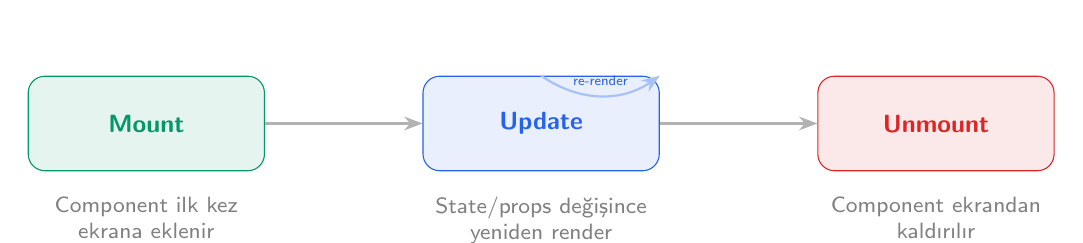
\begin{tikzpicture}[>=Stealth, node distance=1.2cm]

  \node[draw=accent, fill=accent!10, rounded corners=6pt,
        minimum width=3.0cm, minimum height=1.2cm,
        font=\sffamily\bfseries\small, text=accent] (mount)
        {Mount};

  \node[draw=primary, fill=primary!10, rounded corners=6pt,
        minimum width=3.0cm, minimum height=1.2cm,
        font=\sffamily\bfseries\small, text=primary,
        right=2.0cm of mount] (update)
        {Update};

  \node[draw=danger, fill=danger!10, rounded corners=6pt,
        minimum width=3.0cm, minimum height=1.2cm,
        font=\sffamily\bfseries\small, text=danger,
        right=2.0cm of update] (unmount)
        {Unmount};

  \node[font=\sffamily\footnotesize, text=gray, below=0.2cm of mount, align=center]
    {Component ilk kez\\ekrana eklenir};
  \node[font=\sffamily\footnotesize, text=gray, below=0.2cm of update, align=center]
    {State/props değişince\\yeniden render};
  \node[font=\sffamily\footnotesize, text=gray, below=0.2cm of unmount, align=center]
    {Component ekrandan\\kaldırılır};

  \draw[->, thick, gray!60] (mount) -- (update);
  \draw[->, thick, gray!60] (update) -- (unmount);
  \draw[->, thick, primary!40, bend right=35]
    (update.north) to node[above, font=\sffamily\tiny, text=primary] {re-render} (update.north east);

\end{tikzpicture}
\end{center}

\vspace{6pt}

\begin{definebox}[useEffect Nedir?]
\texttt{useEffect}, component'in \textbf{yan etkilerini} (side effects) yönetmek
için kullanılan React Hook'udur. Yan etki = render dışında olan her şey:
\begin{itemize}
  \item API'den veri çekme (fetch)
  \item DOM manipülasyonu
  \item Timer (setTimeout, setInterval)
  \item Event listener ekleme/kaldırma
  \item localStorage okuma/yazma
\end{itemize}
\end{definebox}

% ----------------------------------------------------------
\subsection{useEffect Söz Dizimi}

\begin{tcolorbox}[enhanced, colback=codebg, colframe=gray!30,
    colbacktitle=primary!85!black, coltitle=white, arc=4pt,
    title={\sffamily\bfseries\small useEffect Formülü}]
\begin{lstlisting}[style=jsxstyle]
import { useEffect } from "react";

useEffect(() => {
  // Yan etki burada calisir

  return () => {
    // Cleanup (temizlik) --- opsiyonel
  };
}, [bagimliliklar]); // dependency array
\end{lstlisting}
\end{tcolorbox}

\vspace{6pt}

\subsubsection{Dependency Array Davranışları}

\begin{tcolorbox}[enhanced, colback=lightbg, colframe=gray!30, arc=4pt]
\sffamily\small
\begin{tabularx}{\textwidth}{>{\ttfamily\color{primary}}l X >{\color{secondary}\itshape}l}
\toprule
\normalfont\bfseries Kullanım & \normalfont\bfseries Ne Zaman Çalışır? & \normalfont\bfseries Benzetme \\
\midrule
useEffect(() => \{\}, [])       & Sadece ilk render'da (mount) & componentDidMount \\[4pt]
useEffect(() => \{\}, [a, b])   & İlk render + a veya b değişince & componentDidUpdate \\[4pt]
useEffect(() => \{\})           & Her render'da (genellikle istemezsiniz!) & --- \\[4pt]
return () => \{\}               & Unmount veya effect tekrar çalışmadan önce & componentWillUnmount \\
\bottomrule
\end{tabularx}
\end{tcolorbox}

\vspace{8pt}

\begin{tcolorbox}[enhanced, colback=codebg, colframe=gray!30,
    colbacktitle=primary!85!black, coltitle=white, arc=4pt,
    title={\sffamily\bfseries\small Örnek 1 --- Sayfa Başlığını Güncelleme}]
\begin{lstlisting}[style=jsxstyle]
import { useState, useEffect } from "react";

function Counter() {
  const [count, setCount] = useState(0);

  // count degisince sayfa basligini guncelle
  useEffect(() => {
    document.title = `Count: ${count}`;
  }, [count]);

  return (
    <div>
      <p>{count}</p>
      <button onClick={() => setCount(count + 1)}>
        +1
      </button>
    </div>
  );
}
\end{lstlisting}
\end{tcolorbox}

\vspace{6pt}

\begin{tcolorbox}[enhanced, colback=codebg, colframe=gray!30,
    colbacktitle=primary!85!black, coltitle=white, arc=4pt,
    title={\sffamily\bfseries\small Örnek 2 --- API'den Veri Çekme (En Yaygın Kullanım)}]
\begin{lstlisting}[style=jsxstyle]
import { useState, useEffect } from "react";

function UserList() {
  const [users, setUsers] = useState([]);
  const [loading, setLoading] = useState(true);

  useEffect(() => {
    async function fetchUsers() {
      const res = await fetch(
        "https://jsonplaceholder.typicode.com/users"
      );
      const data = await res.json();
      setUsers(data);
      setLoading(false);
    }

    fetchUsers();
  }, []); // bos dizi = sadece mount'ta calis

  if (loading) return <p>Loading...</p>;

  return (
    <ul>
      {users.map(user => (
        <li key={user.id}>{user.name}</li>
      ))}
    </ul>
  );
}
\end{lstlisting}
\end{tcolorbox}

% ----------------------------------------------------------
\newpage
\subsection{Cleanup (Temizlik) Fonksiyonu}

Bazı yan etkiler temizlenmezse \textbf{memory leak} (bellek sızıntısı) oluşur.
Örneğin timer veya event listener eklediysek, component kaldırılınca bunları
temizlemeliyiz.

\vspace{6pt}

\begin{tcolorbox}[enhanced, colback=codebg, colframe=gray!30,
    colbacktitle=primary!85!black, coltitle=white, arc=4pt,
    title={\sffamily\bfseries\small Cleanup --- Timer Örneği}]
\begin{lstlisting}[style=jsxstyle]
import { useState, useEffect } from "react";

function Timer() {
  const [seconds, setSeconds] = useState(0);

  useEffect(() => {
    const interval = setInterval(() => {
      setSeconds(prev => prev + 1);
    }, 1000);

    // Cleanup: component unmount olunca timer'i durdur
    return () => clearInterval(interval);
  }, []);

  return <p>Elapsed: {seconds}s</p>;
}
\end{lstlisting}
\end{tcolorbox}

\vspace{8pt}

\begin{center}
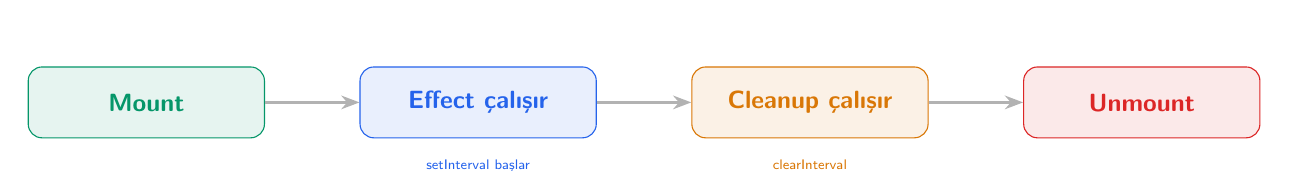
\begin{tikzpicture}[>=Stealth, node distance=1.0cm]

  \node[draw=accent, fill=accent!10, rounded corners=5pt,
        minimum width=3.0cm, minimum height=0.9cm,
        font=\sffamily\bfseries\small, text=accent] (mount)
        {Mount};

  \node[draw=primary, fill=primary!10, rounded corners=5pt,
        minimum width=3.0cm, minimum height=0.9cm,
        font=\sffamily\small\bfseries, text=primary,
        right=1.2cm of mount] (effect)
        {Effect çalışır};

  \node[draw=warning, fill=warning!10, rounded corners=5pt,
        minimum width=3.0cm, minimum height=0.9cm,
        font=\sffamily\small\bfseries, text=warning,
        right=1.2cm of effect] (cleanup)
        {Cleanup çalışır};

  \node[draw=danger, fill=danger!10, rounded corners=5pt,
        minimum width=3.0cm, minimum height=0.9cm,
        font=\sffamily\small\bfseries, text=danger,
        right=1.2cm of cleanup] (unmount)
        {Unmount};

  \draw[->, thick, gray!60] (mount) -- (effect);
  \draw[->, thick, gray!60] (effect) -- (cleanup);
  \draw[->, thick, gray!60] (cleanup) -- (unmount);

  \node[font=\sffamily\tiny, text=primary, below=0.15cm of effect]
    {setInterval başlar};
  \node[font=\sffamily\tiny, text=warning, below=0.15cm of cleanup]
    {clearInterval};

\end{tikzpicture}
\end{center}

\vspace{6pt}

\begin{warningbox}[\faExclamationTriangle\ Sık Yapılan Hatalar]
\begin{enumerate}
  \item \textbf{Dependency array unutmak:} Effect her render'da çalışır,
        sonsuz döngüye girebilir.
  \item \textbf{Bağımlılık eksik bırakmak:} Effect eski (stale) değerlerle çalışır.
  \item \textbf{useEffect içinde doğrudan async fonksiyon:}
        \texttt{useEffect(async () => ...)} \textbf{yazılmaz}.
        İçeride ayrı bir async fonksiyon tanımlayıp çağırın.
\end{enumerate}
\end{warningbox}

% ============================================================
\newpage
\section{\faCodeBranch\ Conditional ve List Rendering}
\timebadge{25--50 dakika}

\subsection{Conditional Rendering (Koşullu Gösterim)}

React'ta bir component'in ne göstereceğini koşullara göre değiştirebiliriz.
Bunun birkaç yolu var:

\vspace{6pt}

\subsubsection{Yöntem 1 --- if / else ile Erken Return}

\begin{tcolorbox}[enhanced, colback=codebg, colframe=gray!30,
    colbacktitle=primary!85!black, coltitle=white, arc=4pt,
    title={\sffamily\bfseries\small if/else --- Erken Return}]
\begin{lstlisting}[style=jsxstyle]
function Dashboard({ isLoggedIn }) {
  if (!isLoggedIn) {
    return <p>Please login first.</p>;
  }

  return <h1>Welcome to Dashboard!</h1>;
}
\end{lstlisting}
\end{tcolorbox}

\vspace{6pt}

\subsubsection{Yöntem 2 --- Ternary Operatör (\texttt{? :})}

\begin{tcolorbox}[enhanced, colback=codebg, colframe=gray!30,
    colbacktitle=primary!85!black, coltitle=white, arc=4pt,
    title={\sffamily\bfseries\small Ternary ile Koşullu Render}]
\begin{lstlisting}[style=jsxstyle]
function Greeting({ isLoggedIn, userName }) {
  return (
    <div>
      {isLoggedIn
        ? <h1>Welcome, {userName}!</h1>
        : <h1>Please sign in.</h1>
      }
    </div>
  );
}
\end{lstlisting}
\end{tcolorbox}

\vspace{6pt}

\subsubsection{Yöntem 3 --- \texttt{\&\&} (Logical AND)}

Sadece bir koşul sağlandığında göstermek istiyorsak:

\begin{tcolorbox}[enhanced, colback=codebg, colframe=gray!30,
    colbacktitle=primary!85!black, coltitle=white, arc=4pt,
    title={\sffamily\bfseries\small \&\& ile Koşullu Render}]
\begin{lstlisting}[style=jsxstyle]
function Notifications({ count }) {
  return (
    <div>
      <h1>Home</h1>
      {count > 0 && (
        <span className="badge">{count} new notifications</span>
      )}
    </div>
  );
}
\end{lstlisting}
\end{tcolorbox}

\vspace{6pt}

\begin{tcolorbox}[enhanced, colback=lightbg, colframe=gray!30, arc=4pt]
\sffamily\small
\begin{tabularx}{\textwidth}{>{\ttfamily\bfseries\color{primary}}l X >{\color{secondary}}l}
\toprule
\normalfont\bfseries Yöntem & \normalfont\bfseries Ne Zaman? & \normalfont\bfseries Örnek \\
\midrule
if / return   & Tamamen farklı UI döndürme & Loading / Error / Data \\
? :           & İki alternatif arasında seçim & Login / Logout butonu \\
\&\&          & Bir şeyi göster \textbf{veya hiç gösterme} & Badge, uyarı mesajı \\
\bottomrule
\end{tabularx}
\end{tcolorbox}

\vspace{6pt}

\begin{dangerbox}[\faExclamationCircle\ \texttt{\&\&} ile Sıfır Tuzağı]
\texttt{\{count \&\& <span>\{count\}</span>\}} yazdığınızda,
\texttt{count} sıfırsa ekranda \texttt{0} görünür (false değil!).
Çözüm: \texttt{\{count > 0 \&\& ...\}} şeklinde açıkça boolean karşılaştırma yapın.
\end{dangerbox}

% ----------------------------------------------------------
\newpage
\subsection{Gerçekçi Örnek --- Loading / Error / Data Patterni}

API çağrılarında en yaygın conditional rendering kalıbı:

\vspace{6pt}

\begin{tcolorbox}[enhanced, colback=codebg, colframe=gray!30,
    colbacktitle=primary!85!black, coltitle=white, arc=4pt,
    title={\sffamily\bfseries\small Loading / Error / Data}]
\begin{lstlisting}[style=jsxstyle]
function ProductList() {
  const [products, setProducts] = useState([]);
  const [loading, setLoading] = useState(true);
  const [error, setError] = useState(null);

  useEffect(() => {
    async function fetchProducts() {
      try {
        const res = await fetch("/api/products");
        if (!res.ok) throw new Error("Failed to fetch");
        const data = await res.json();
        setProducts(data);
      } catch (err) {
        setError(err.message);
      } finally {
        setLoading(false);
      }
    }
    fetchProducts();
  }, []);

  if (loading) return <p>Loading...</p>;
  if (error)   return <p className="error">{error}</p>;
  if (products.length === 0) return <p>No products found.</p>;

  return (
    <ul>
      {products.map(p => (
        <li key={p.id}>{p.name} - {p.price} TL</li>
      ))}
    </ul>
  );
}
\end{lstlisting}
\end{tcolorbox}

% ----------------------------------------------------------
\subsection{List Rendering ve \texttt{key} Prop'u}

\subsubsection{map ile Liste Render}

React'ta bir diziyi UI'a dönüştürmek için \texttt{map} kullanılır:

\vspace{6pt}

\begin{tcolorbox}[enhanced, colback=codebg, colframe=gray!30,
    colbacktitle=primary!85!black, coltitle=white, arc=4pt,
    title={\sffamily\bfseries\small Liste Render Örneği}]
\begin{lstlisting}[style=jsxstyle]
const fruits = ["Apple", "Banana", "Cherry"];

function FruitList() {
  return (
    <ul>
      {fruits.map((fruit, index) => (
        <li key={index}>{fruit}</li>
      ))}
    </ul>
  );
}
\end{lstlisting}
\end{tcolorbox}

\vspace{6pt}

\subsubsection{key Neden Önemli?}

React, listedeki hangi elemanın eklendiğini, silindiğini veya değiştiğini
anlamak için \texttt{key} prop'unu kullanır. \texttt{key} olmazsa React
tüm listeyi baştan render eder.

\vspace{8pt}

\begin{center}
\begin{tikzpicture}[>=Stealth]

  % Sol: key olmadan
  \node[font=\sffamily\bfseries\small, text=danger] at (0, 4.4) {key yok / index key:};

  \fill[danger!15] (-0.8, 3.0) rectangle (3.3, 4.0);
  \node[font=\sffamily\tiny, text=danger] at (1.25, 3.5) {Yeni eleman eklendi};

  \fill[danger!25] (-0.8, 2.0) rectangle (3.3, 2.8);
  \node[font=\sffamily\tiny] at (1.25, 2.4) {Tüm liste yeniden render};
  \node[font=\sffamily\tiny, text=danger] at (1.25, 1.6) {\faTimesCircle\ Yavaş + state kaybı riski};

  % Sağ: key ile
  \node[font=\sffamily\bfseries\small, text=accent] at (6.0, 4.4) {Benzersiz key:};

  \fill[accent!15] (5.2, 3.0) rectangle (9.3, 4.0);
  \node[font=\sffamily\tiny, text=accent] at (7.25, 3.5) {Yeni eleman eklendi};

  \fill[accent!15] (5.2, 2.0) rectangle (7.0, 2.8);
  \node[font=\sffamily\tiny] at (6.1, 2.4) {Sadece yeni};

  \fill[gray!10] (7.2, 2.0) rectangle (9.3, 2.8);
  \node[font=\sffamily\tiny, text=gray] at (8.25, 2.4) {Dokunulmaz};
  \node[font=\sffamily\tiny, text=accent] at (7.25, 1.6) {\faCheckCircle\ Hızlı + state korunur};

\end{tikzpicture}
\end{center}

\vspace{6pt}

\begin{warningbox}[\faExclamationTriangle\ key Kuralları]
\begin{itemize}
  \item \texttt{key} \textbf{benzersiz ve sabit} olmalıdır (veritabanı \texttt{id} idealdir).
  \item \texttt{index} son çare olarak kullanılabilir --- sıralama veya silme
        yapılan listelerde \textbf{sorun yaratır}.
  \item \texttt{key} bir prop değildir; component içinden \texttt{props.key}
        ile erişilemez.
  \item \texttt{key} sadece kardeş elemanlar arasında benzersiz olmalıdır,
        global benzersizlik gerekmez.
\end{itemize}
\end{warningbox}

\vspace{6pt}

\begin{tcolorbox}[enhanced, colback=codebg, colframe=gray!30,
    colbacktitle=primary!85!black, coltitle=white, arc=4pt,
    title={\sffamily\bfseries\small Doğru key Kullanımı}]
\begin{lstlisting}[style=jsxstyle]
const users = [
  { id: 1, name: "Ali" },
  { id: 2, name: "Veli" },
  { id: 3, name: "Zeynep" },
];

function UserList() {
  return (
    <ul>
      {users.map(user => (
        <li key={user.id}>{user.name}</li>
      ))}
    </ul>
  );
}
\end{lstlisting}
\end{tcolorbox}

% ============================================================
\newpage
\section{\faKeyboard\ Form Handling ve Validation}
\timebadge{50--75 dakika}

\subsection{Controlled Component (Hatırlatma)}

Session~3'te öğrendiğimiz gibi, React'ta input'ların değeri \textbf{state'te}
tutulur. Bu yaklaşıma \textbf{controlled component} denir.

\vspace{6pt}

\begin{center}
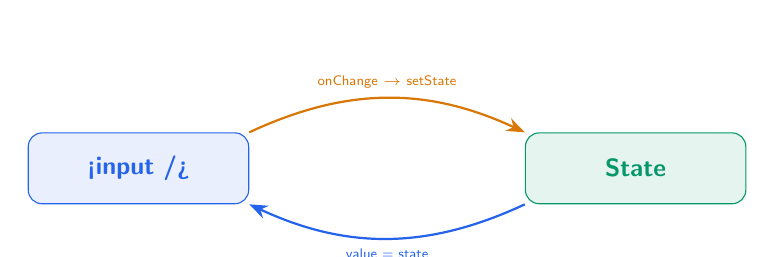
\begin{tikzpicture}[>=Stealth]

  \node[draw=primary, fill=primary!10, rounded corners=5pt,
        minimum width=2.8cm, minimum height=0.9cm,
        font=\sffamily\small\bfseries, text=primary] (input)
        {<input />};

  \node[draw=accent, fill=accent!10, rounded corners=5pt,
        minimum width=2.8cm, minimum height=0.9cm,
        font=\sffamily\small\bfseries, text=accent,
        right=3.5cm of input] (state)
        {State};

  \draw[->, thick, warning, bend left=25]
    (input.north east) to
    node[above, font=\sffamily\tiny, text=warning] {onChange $\rightarrow$ setState}
    (state.north west);

  \draw[->, thick, primary, bend left=25]
    (state.south west) to
    node[below, font=\sffamily\tiny, text=primary] {value = state}
    (input.south east);

\end{tikzpicture}
\end{center}

% ----------------------------------------------------------
\subsection{Form Submit}

Form gönderimi için \texttt{onSubmit} event'i kullanılır.
\texttt{e.preventDefault()} ile sayfanın yenilenmesini önleriz.

\vspace{6pt}

\begin{tcolorbox}[enhanced, colback=codebg, colframe=gray!30,
    colbacktitle=primary!85!black, coltitle=white, arc=4pt,
    title={\sffamily\bfseries\small Form Submit Örneği}]
\begin{lstlisting}[style=jsxstyle]
import { useState } from "react";

function LoginForm() {
  const [email, setEmail] = useState("");
  const [password, setPassword] = useState("");

  const handleSubmit = (e) => {
    e.preventDefault(); // sayfa yenilenmesin

    console.log("Email:", email);
    console.log("Password:", password);
    // API cagrisi yapilabilir
  };

  return (
    <form onSubmit={handleSubmit}>
      <label htmlFor="email">Email:</label>
      <input
        id="email"
        type="email"
        value={email}
        onChange={(e) => setEmail(e.target.value)}
      />

      <label htmlFor="password">Password:</label>
      <input
        id="password"
        type="password"
        value={password}
        onChange={(e) => setPassword(e.target.value)}
      />

      <button type="submit">Login</button>
    </form>
  );
}
\end{lstlisting}
\end{tcolorbox}

% ----------------------------------------------------------
\newpage
\subsection{Birden Fazla Input --- Tek State Objesi}

Çok sayıda input varsa her biri için ayrı state yerine
tek bir \textbf{obje state} kullanmak daha pratiktir:

\vspace{6pt}

\begin{tcolorbox}[enhanced, colback=codebg, colframe=gray!30,
    colbacktitle=primary!85!black, coltitle=white, arc=4pt,
    title={\sffamily\bfseries\small Obje State ile Çoklu Input}]
\begin{lstlisting}[style=jsxstyle]
import { useState } from "react";

function RegisterForm() {
  const [form, setForm] = useState({
    name: "",
    email: "",
    password: "",
  });

  const handleChange = (e) => {
    const { name, value } = e.target;
    setForm(prev => ({
      ...prev,        // onceki degerleri koru
      [name]: value,  // sadece degisen alani guncelle
    }));
  };

  const handleSubmit = (e) => {
    e.preventDefault();
    console.log("Form data:", form);
  };

  return (
    <form onSubmit={handleSubmit}>
      <input name="name"     value={form.name}
             onChange={handleChange} placeholder="Name" />
      <input name="email"    value={form.email}
             onChange={handleChange} placeholder="Email" />
      <input name="password" value={form.password}
             onChange={handleChange} placeholder="Password"
             type="password" />
      <button type="submit">Register</button>
    </form>
  );
}
\end{lstlisting}
\end{tcolorbox}

\vspace{6pt}

\begin{infobox}[\faLightbulb\ Computed Property Name]
\texttt{[name]: value} söz dizimi JavaScript'in
\textbf{computed property name} özelliğidir. \texttt{name} değişkeninin
değeri ne ise o key güncellenir. Session~2'deki destructuring ve
spread bilgisi burada devreye giriyor.
\end{infobox}

% ----------------------------------------------------------
\subsection{Basic Validation (Temel Doğrulama)}

Form gönderilmeden önce verilerin geçerliliğini kontrol etmemiz gerekir.
En basit yaklaşım: submit anında kontrol et, hata varsa göster.

\vspace{6pt}

\begin{tcolorbox}[enhanced, colback=codebg, colframe=gray!30,
    colbacktitle=primary!85!black, coltitle=white, arc=4pt,
    title={\sffamily\bfseries\small Temel Validation}]
\begin{lstlisting}[style=jsxstyle]
import { useState } from "react";

function ContactForm() {
  const [name, setName] = useState("");
  const [email, setEmail] = useState("");
  const [errors, setErrors] = useState({});

  const validate = () => {
    const newErrors = {};
    if (!name.trim()) newErrors.name = "Name is required";
    if (!email.trim()) {
      newErrors.email = "Email is required";
    } else if (!email.includes("@")) {
      newErrors.email = "Invalid email";
    }
    return newErrors;
  };

  const handleSubmit = (e) => {
    e.preventDefault();
    const validationErrors = validate();

    if (Object.keys(validationErrors).length > 0) {
      setErrors(validationErrors);
      return; // gondermeden dur
    }

    setErrors({});
    console.log("Form submitted:", { name, email });
  };

  return (
    <form onSubmit={handleSubmit}>
      <input value={name}
             onChange={(e) => setName(e.target.value)}
             placeholder="Name" />
      {errors.name && (
        <span className="error">{errors.name}</span>
      )}

      <input value={email}
             onChange={(e) => setEmail(e.target.value)}
             placeholder="Email" />
      {errors.email && (
        <span className="error">{errors.email}</span>
      )}

      <button type="submit">Send</button>
    </form>
  );
}
\end{lstlisting}
\end{tcolorbox}

\vspace{6pt}

\begin{tcolorbox}[enhanced, colback=lightbg, colframe=gray!30, arc=4pt]
\sffamily\small
\begin{tabularx}{\textwidth}{>{\bfseries\color{primary}}l X}
\toprule
Yaklaşım & Açıklama \\
\midrule
Submit validation &
  Form gönderildiğinde kontrol et. Basit ve anlaşılır. \\[4pt]
onChange validation &
  Her tuş vuruşunda kontrol et. Anlık geri bildirim ama daha fazla kod. \\[4pt]
onBlur validation &
  Input'tan çıkınca kontrol et. İkisinin arası --- kullanıcı dostu. \\
\bottomrule
\end{tabularx}
\end{tcolorbox}

% ============================================================
\newpage
\section{\faHammer\ Pratik: Mini ToDo Uygulaması}
\timebadge{75--90 dakika}

\begin{practicebox}[\faTasks\ Pratik Hedef]
Bu session'da öğrendiğimiz her şeyi birleştirerek bir \textbf{ToDo uygulaması}
yazacağız:
\begin{enumerate}
  \item Yeni görev ekleme (form + validation)
  \item Görev listesi render etme (map + key)
  \item Görevi tamamlandı olarak işaretleme (conditional rendering)
  \item Görevi silme (filter ile state güncelleme)
  \item Kalan görev sayısını gösterme
\end{enumerate}
\end{practicebox}

\vspace{8pt}

\begin{tcolorbox}[enhanced, colback=codebg, colframe=gray!30,
    colbacktitle=primary!85!black, coltitle=white, arc=4pt,
    title={\sffamily\bfseries\small TodoApp.jsx}]
\begin{lstlisting}[style=jsxstyle]
import { useState } from "react";

function TodoApp() {
  const [todos, setTodos] = useState([]);
  const [text, setText] = useState("");
  const [error, setError] = useState("");

  // --- Ekleme ---
  const handleAdd = (e) => {
    e.preventDefault();

    if (!text.trim()) {
      setError("Task cannot be empty!");
      return;
    }

    const newTodo = {
      id: Date.now(),
      text: text.trim(),
      completed: false,
    };

    setTodos([...todos, newTodo]);
    setText("");
    setError("");
  };

  // --- Tamamlandi/geri al ---
  const toggleTodo = (id) => {
    setTodos(
      todos.map(todo =>
        todo.id === id
          ? { ...todo, completed: !todo.completed }
          : todo
      )
    );
  };

  // --- Silme ---
  const deleteTodo = (id) => {
    setTodos(todos.filter(todo => todo.id !== id));
  };

  const remaining = todos.filter(t => !t.completed).length;
\end{lstlisting}
\end{tcolorbox}

\vspace{4pt}

\begin{tcolorbox}[enhanced, colback=codebg, colframe=gray!30,
    colbacktitle=primary!85!black, coltitle=white, arc=4pt,
    title={\sffamily\bfseries\small TodoApp.jsx (devam --- return kısmı)}]
\begin{lstlisting}[style=jsxstyle]
  return (
    <div style={{ maxWidth: 500, margin: "40px auto" }}>
      <h1>My Todos</h1>

      {/* --- Form --- */}
      <form onSubmit={handleAdd}>
        <input
          type="text"
          value={text}
          onChange={(e) => setText(e.target.value)}
          placeholder="What needs to be done?"
        />
        <button type="submit">Add</button>
      </form>
      {error && <p style={{ color: "red" }}>{error}</p>}

      {/* --- Liste --- */}
      <ul style={{ listStyle: "none", padding: 0 }}>
        {todos.map(todo => (
          <li key={todo.id}
              style={{
                textDecoration: todo.completed
                  ? "line-through" : "none",
                color: todo.completed
                  ? "#94a3b8" : "#1e293b",
              }}>

            <input type="checkbox"
                   checked={todo.completed}
                   onChange={() => toggleTodo(todo.id)} />

            <span>{todo.text}</span>

            <button onClick={() => deleteTodo(todo.id)}>
              Delete
            </button>
          </li>
        ))}
      </ul>

      {/* --- Ozet --- */}
      {todos.length > 0 && (
        <p>{remaining} task(s) remaining</p>
      )}
    </div>
  );
}

export default TodoApp;
\end{lstlisting}
\end{tcolorbox}

\vspace{8pt}

\begin{infobox}[\faLightbulb\ Bu Kodda Neler Kullandık?]
\begin{itemize}
  \item \texttt{useState} --- 3 farklı state (\texttt{todos}, \texttt{text}, \texttt{error})
  \item \texttt{onSubmit} + \texttt{e.preventDefault()} --- form gönderimi
  \item \texttt{validation} --- boş görev eklemeyi engelleme
  \item \texttt{map} ile liste render + \texttt{key=\{todo.id\}}
  \item \texttt{filter} ile silme (immutable güncelleme)
  \item \texttt{spread} ile toggle (\texttt{\{...todo, completed: !todo.completed\}})
  \item \texttt{ternary} ile koşullu stil
  \item \texttt{\&\&} ile koşullu gösterim (özet satırı)
\end{itemize}
\end{infobox}

\vspace{6pt}

\begin{warningbox}[\faExclamationTriangle\ Immutable Güncelleme]
React'ta state \textbf{doğrudan değiştirilmez}. Diziden silmek için
\texttt{splice} yerine \texttt{filter}, güncellemek için doğrudan
atama yerine \texttt{map + spread} kullanırız. Bu sayede React
değişiklikleri algılar ve ekranı günceller.

\vspace{4pt}
\texttt{todos.splice(i, 1)} \quad\color{danger}\faTimes\ Yanlış --- orijinal diziyi değiştirir

\texttt{todos.filter(t => t.id !== id)} \quad\color{accent}\faCheck\ Doğru --- yeni dizi döndürür
\end{warningbox}

% ============================================================
\newpage
\section{\faCheckCircle\ Özet ve Sonraki Session}

\subsection{Bu Session'da Öğrendiklerimiz}

\begin{tcolorbox}[enhanced, colback=lightbg, colframe=gray!30, arc=4pt]
\begin{itemize}
  \item[\color{accent}\faCheck] Component lifecycle: mount, update, unmount
  \item[\color{accent}\faCheck] \texttt{useEffect} ile yan etki yönetimi
  \item[\color{accent}\faCheck] Dependency array: \texttt{[]}, \texttt{[a, b]}, hiç verilmezse ne olur
  \item[\color{accent}\faCheck] Cleanup fonksiyonu ve memory leak önleme
  \item[\color{accent}\faCheck] Conditional rendering: if/return, ternary (\texttt{? :}), \texttt{\&\&}
  \item[\color{accent}\faCheck] Loading / Error / Data patterni
  \item[\color{accent}\faCheck] List rendering: \texttt{map} ile dizi $\rightarrow$ UI
  \item[\color{accent}\faCheck] \texttt{key} prop'unun önemi ve doğru kullanımı
  \item[\color{accent}\faCheck] Form handling: \texttt{onSubmit}, \texttt{e.preventDefault()}
  \item[\color{accent}\faCheck] Obje state ile çoklu input yönetimi
  \item[\color{accent}\faCheck] Temel form validation
  \item[\color{accent}\faCheck] Pratik: Mini ToDo uygulaması (CRUD)
\end{itemize}
\end{tcolorbox}

\vspace{6pt}

\subsection{Sıkça Sorulan Sorular}

\begin{warningbox}[\faQuestionCircle\ SSS]
\textbf{S: useEffect her render'da çalışır mı?}\\
C: Dependency array'e bağlı. Boş dizi (\texttt{[]}) verilirse sadece mount'ta,
belirli değerler verilirse o değerler değişince çalışır.
Array hiç verilmezse her render'da çalışır --- bu genellikle istenmez.

\vspace{6pt}
\textbf{S: Neden \texttt{index} yerine \texttt{id} kullanmalıyız?}\\
C: Liste sıralama, ekleme veya silme yapılırsa index değişir; React yanlış
elemanları eşleştirir ve input state'leri kaybolabilir. Sabit bir
\texttt{id} bu sorunu önler.

\vspace{6pt}
\textbf{S: State'i neden spread ile güncelliyoruz?}\\
C: React, referans karşılaştırması yapar. Aynı obje/diziyi mutate edersek
React değişikliği fark edemez. \texttt{spread} ile yeni obje/dizi oluşturmak
React'a ``bu değişti, yeniden render et'' sinyali verir.

\vspace{6pt}
\textbf{S: Form validation için kütüphane kullanmalı mıyız?}\\
C: Basit formlarda el ile yeterlidir. Karmaşık formlar için
\texttt{react-hook-form} veya \texttt{Formik} gibi kütüphaneler
hayatı kolaylaştırır --- bunları ileride göreceğiz.
\end{warningbox}

\vspace{6pt}

\subsection{Sonraki Session --- Session 5: React Best Practices}

\begin{infobox}[\faArrowRight\ Session 5 (7 Mayıs Perşembe)]
Kod kalitesini artırmak ve doğru mimari yaklaşımı öğrenmek için:
\begin{itemize}
  \item \textbf{Component parçalama} ve reusable component mantığı
  \item \textbf{State yönetimi} yaklaşımları: lifting state up, props drilling
  \item \textbf{Custom hooks} ile mantık paylaşımı
  \item \textbf{Pratik:} ToDo uygulamasını refactor etme
\end{itemize}
\end{infobox}

\vspace{16pt}
\begin{center}
  \color{gray}\sffamily\small
  Front-end + Next.js Eğitimi \quad|\quad Session 4 / 8 \quad|\quad 6 Mayıs 2026
\end{center}

\end{document}
